\documentclass{beamer}
\usepackage[utf8]{inputenc}

\begin{document}

\title{Summary of Polson and Sokolov 2018}
\subtitle{Deep Learning for Energy Markets}
\author{David Prentiss}
\institute{OR750-004}
\date{\today}

\frame{\titlepage}

\begin{frame}
  \frametitle{The PJM Interconnection}
  \begin{itemize}
 \item The Pennsylvania--New Jersey--Maryland Interconnection (PTO) is a regional transmission organization (RTO).
    \item It implements a wholesale electricity market for a network of producers and consumers in the Mid-Atlantic.
      \item Its primary purpose is to prevent outages or otherwise unmet demand.
        \item Obligations are exchanged in bilateral contracts, the day-ahead market,
          and the real-time market.
  \end{itemize}
\end{frame}

\begin{frame}
  \frametitle{Local marginal price data}
  \begin{itemize}
  \item Local Marginal Prices (LMP) are price data aggregated for prices in various
  locations and interconnection services is the network.
  \item They reflect the cost of producing and transmitting electricity in the network.
    \item Prices are non-linear because electricity.
      \item This paper proposes a NN to model price extremes.
  \end{itemize}
\end{frame}

\begin{frame}
  \frametitle{Load vs. price}
  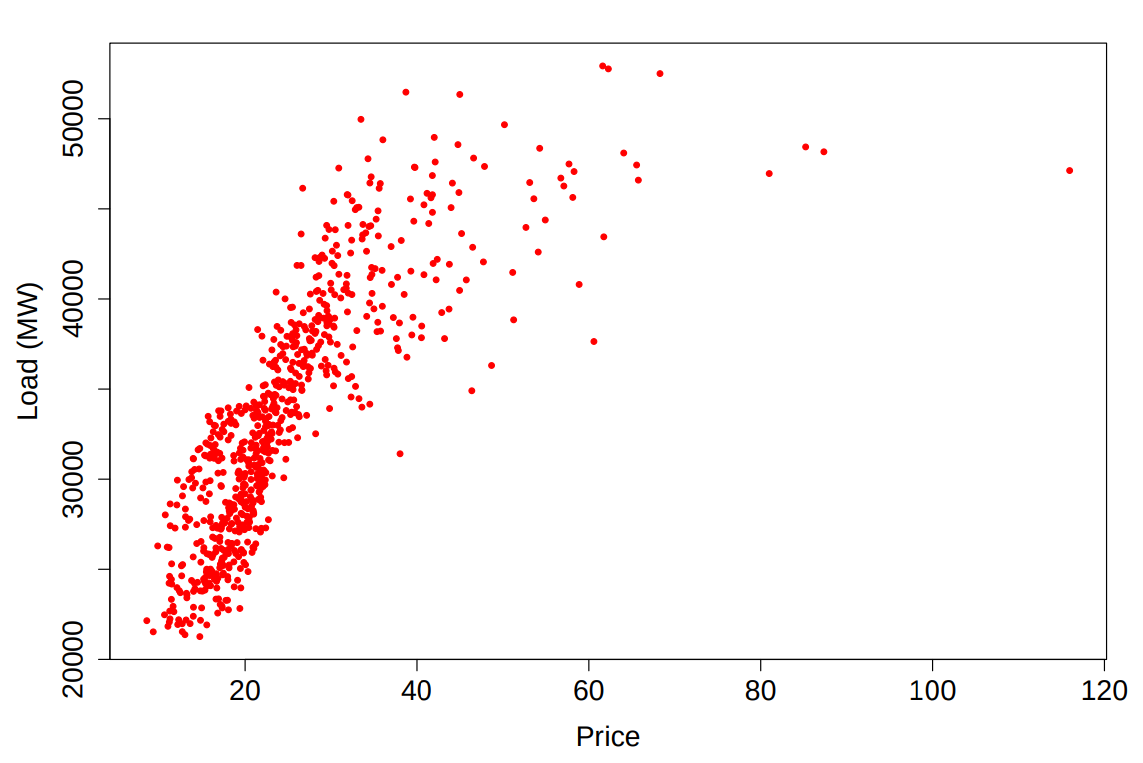
\includegraphics[width=\textwidth]{price.png}
\end{frame}

\begin{frame}
  \frametitle{Load vs. previous load}
  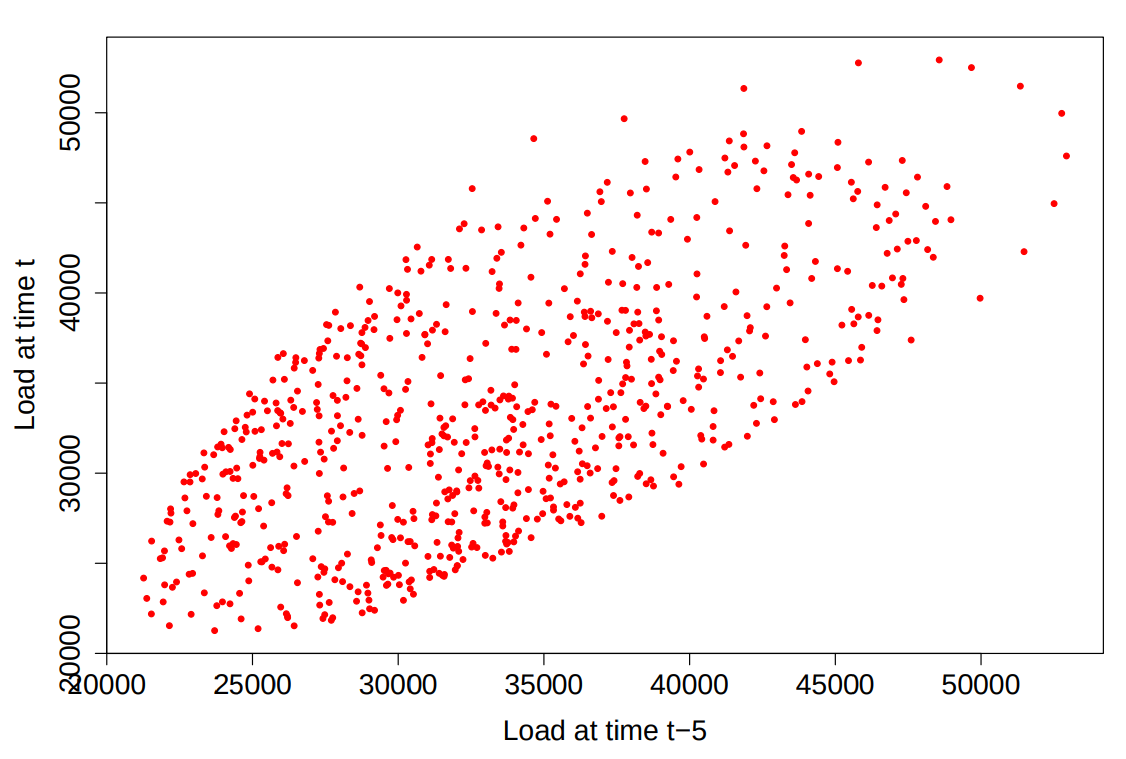
\includegraphics[width=\textwidth]{load.png}
\end{frame}

\begin{frame}
  \frametitle{RNN vs. long short-term memory}
  Vanilla RNN
  \begin{equation*}
    h_t=\tanh\left( W
      \begin{pmatrix}
        h_{t-1} \\ x_t
      \end{pmatrix}
    \right)
  \end{equation*}
  LSTM
  \begin{align*}
    \begin{pmatrix}
      i \\ f \\ o \\ k
    \end{pmatrix}
    &=
    \begin{pmatrix}
      \sigma \\ \sigma \\ \sigma \\ \tanh
    \end{pmatrix}
    \circ
    W
    \begin{pmatrix}
      h_{t-1} \\ x_t
    \end{pmatrix}
    \\
    c_t &= f \odot c_{t-1} + i \odot k \\
    h_t &= o \odot \tanh\left(c_t\right)
  \end{align*}
\end{frame}

\begin{frame}
  \frametitle{LTSM model}
  \begin{align*}
    \begin{pmatrix}
      i \\ f \\ o \\ k
    \end{pmatrix}
    &=
    \begin{pmatrix}
      \sigma \\ \sigma \\ \sigma \\ \tanh
    \end{pmatrix}
    \circ
    W
    \begin{pmatrix}
      h_{t-1} \\ x_t
    \end{pmatrix}
    \\
    c_t &= f \odot c_{t-1} + i \odot k \\
    h_t &= o \odot \tanh\left(c_t\right)
  \end{align*}
  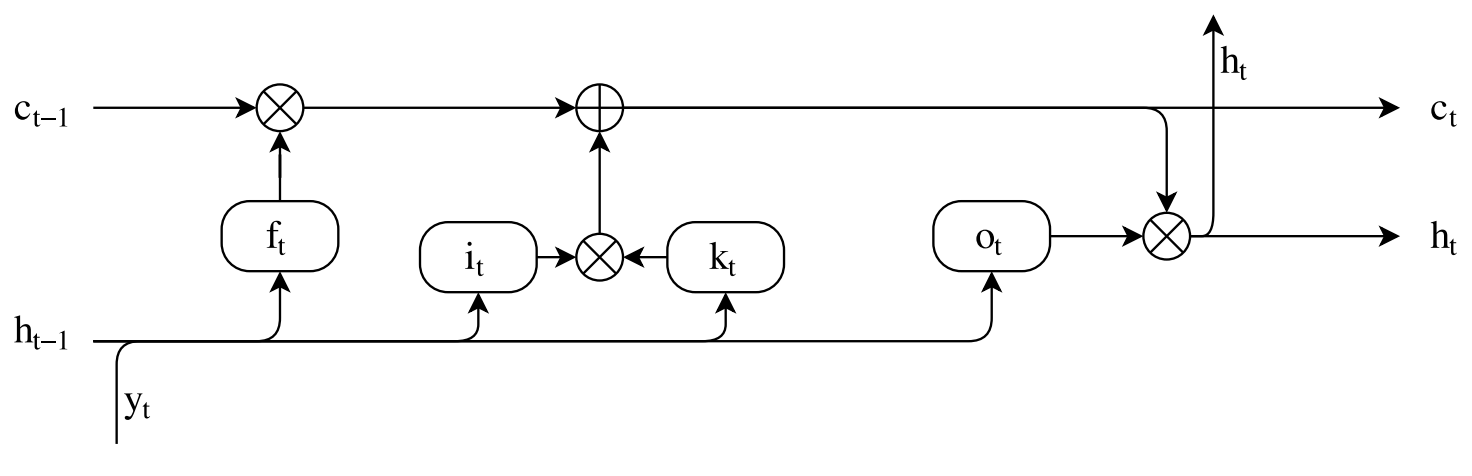
\includegraphics[width=\textwidth]{model.png}
\end{frame}

\begin{frame}
  \frametitle{Extreme value theory}
  \begin{itemize}
  \item Extreme value analysis begins by filtering the data to select
    ``extreme'' values.
    \item Extreme values are selected by one of two methods.
  \begin{itemize}
  \item Block maxima: Select the peak values after dividing the series into periods.
  \item Peak over threshold: Select values larger than some threshold.
  \end{itemize}
    \item Peak over threshold used in this paper.
  \end{itemize}
\end{frame}

\begin{frame}
  \frametitle{Peak over threshold}
  \begin{itemize}
    \item Pickands--Balkema--de Hann (1974 and 1975) theorem characterizes the asymptotic
      tail distribution of an unknown distribution.
      \item Distribution of events that exceed a threshold are approximated with
        the generalized Pareto distribution.
      \item Low threshold increases bias.
      \item High threshold increases variance.
  \end{itemize}
\end{frame}

\begin{frame}
  \frametitle{Generalized Pareto distribution}
  \begin{itemize}
  \item CDF
    \begin{equation*}
      H(y\mid\sigma,\xi)
      =
      1-\left(1+\xi\frac{y-u}{\sigma}\right)_+^{\frac{-1}{\xi}}
    \end{equation*}
  \item PDF
    \begin{equation*}
      h(y\mid\sigma,\xi)
      =
      1-\frac{1}{\sigma}\left(1+\xi\frac{y-u}{\sigma}\right)^{\frac{-1}{\xi}-1}
    \end{equation*}
  \end{itemize}
\end{frame}

\begin{frame}
  \frametitle{Parameters and loss}
    \begin{equation*}
      h(y\mid\sigma,\xi)
      =
      1-\frac{1}{\sigma}\left(1+\xi\frac{y-u}{\sigma}\right)^{\frac{-1}{\xi}-1}
    \end{equation*}
  \begin{itemize}
  \item Location, \(u\), is the threshold
  \item Scale, \(\sigma\), is our learned parameter
  \item Shape, \(\xi = f(u, \sigma)\)?
    \(\text{EX}\left[y\right] = \sigma+u \implies \xi = 0\)?
\item Log-likelihood
  \begin{equation*}
    \log\sigma(t)-(1/\xi+1)\log(1+\sigma(t)\xi(y-u))
    \end{equation*}
    \item Loss function for SGD
      \begin{equation*}
        L(W) = -\frac{1}{n}\sum_{i=1}^n l(y_i\mid x_i, \xi, u, W, b)
      \end{equation*}
  \end{itemize}
\end{frame}

\begin{frame}
  \frametitle{Fourier (ARIMA) model}
  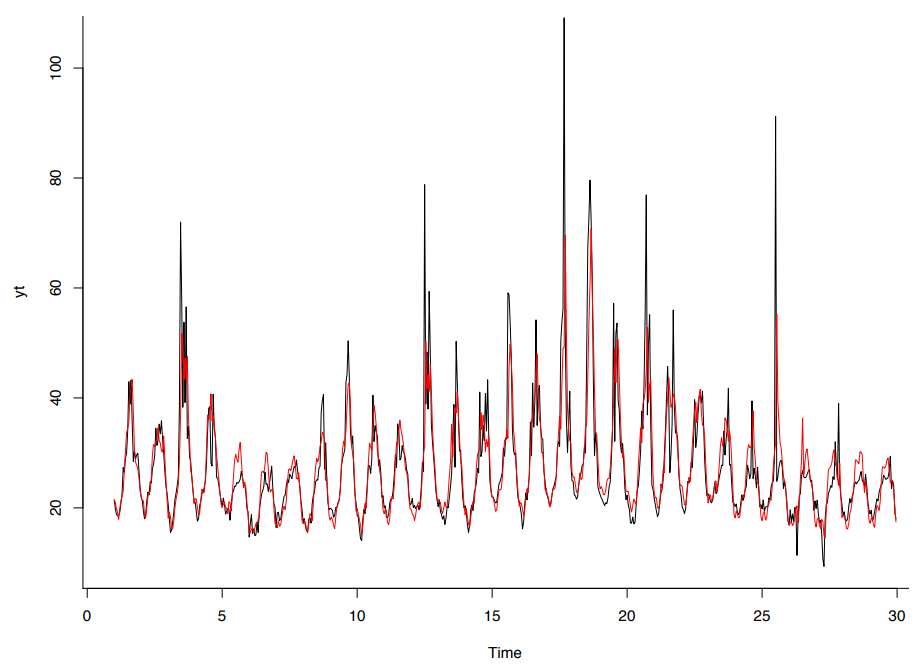
\includegraphics[width=\textwidth]{fourier.png}
\end{frame}

\begin{frame}
  \frametitle{Fourier (ARIMA) model vs DL}
  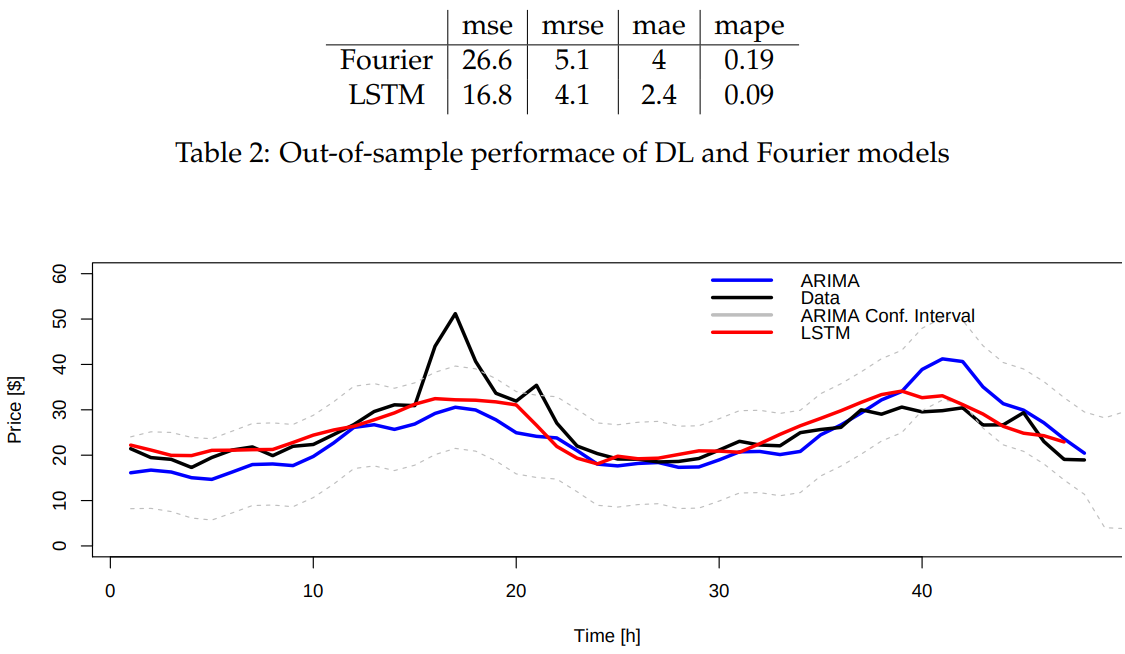
\includegraphics[width=\textwidth]{comp.png}
\end{frame}

\begin{frame}
  \frametitle{Demand forcasting DL--EVT}
  \begin{itemize}
    \item DL--EVT Architecture
      \begin{equation*}
        X\rightarrow\tanh\left(W^{(1)}X+b^{(1)}\right)\rightarrow Z^{(1)}
        \rightarrow\exp\left(\tanh\left(Z^{(1)}\right\right)\rightarrow
        \sigma(X)
      \end{equation*}
    \item \(W^{(1)}\in\mathbb{R}^{p\times 3}\), \(x\in\mathbb{R}^{p}\),
      \(p=24\) (one day)
      \item Threshold, \(u = 31,000\)
  \end{itemize}
\end{frame}

\begin{frame}
  \frametitle{Vanilla DL vs. DL-EVT}
  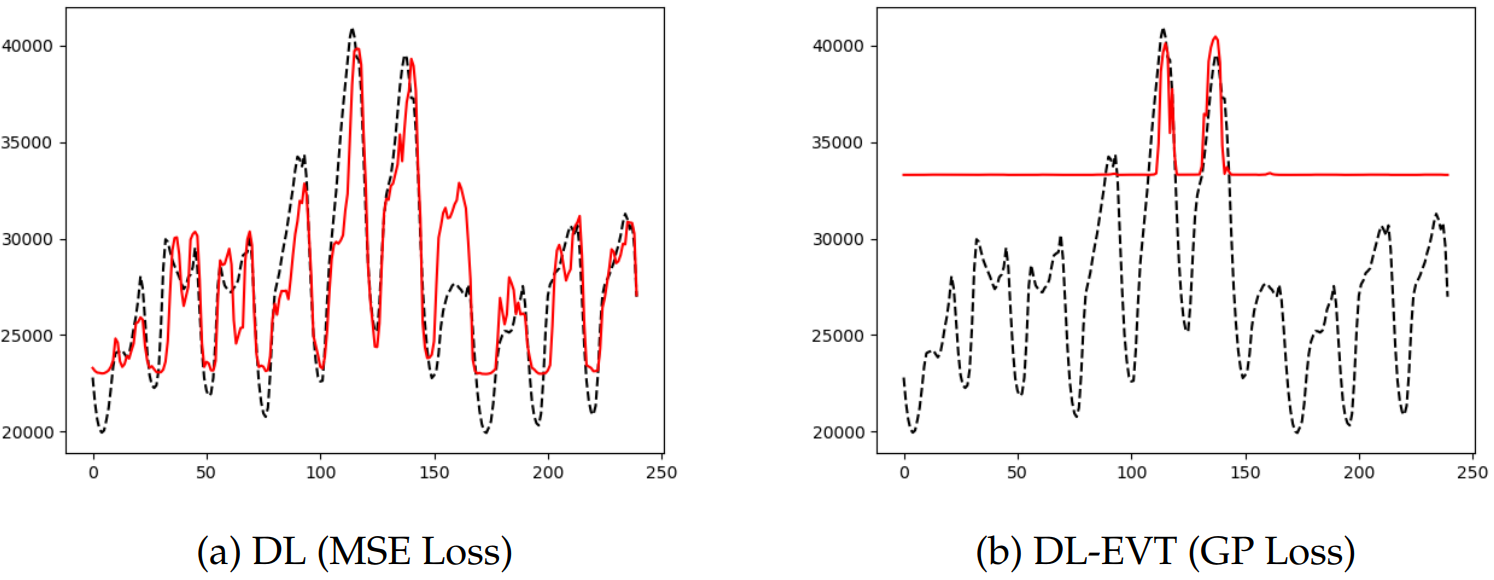
\includegraphics[width=\textwidth]{result.png}
\end{frame}

\end{document}